\title{\textbf{Performer: Fast Attention via Positive Orthogonal Random Features (FAVOR+) for Pretrained Transformers}}

\author{Anonymous authors}



\section{Introduction}

\subsection{Motivation}

Softmax attention scales as $\mathcal{O}(L^2)$ because it materializes the 
$L \times L$ attention matrix. For $L = 8192$, this is 64M entries -- 
infeasible in memory. Linear attention approximates softmax by reordering 
the computation:

\[
\text{Attn}(Q_i, K, V) = \frac{\phi(q_i)^\top \sum_j \phi(k_j) v_j^\top}{\phi(q_i)^\top \sum_j \phi(k_j)}
\tag{1.1}
\]

The sums can be precomputed once, reducing cost to $\mathcal{O}(L d^2)$. The 
challenge is \textbf{choosing the feature map $\phi$} so the approximation is 
accurate.

\subsection{The Performer's FAVOR+ Approach}

Performer (Choromanski et al., 2021) proposes \textbf{FAVOR+} (\textbf{F}ast 
\textbf{A}ttention \textbf{V}ia \textbf{O}rthogonal \textbf{R}andom features). The kernel 
$\exp(q^\top k)$ is approximated by:

\[
\phi(x) = \frac{1}{\sqrt{F}} \exp\!\left(\omega^\top x - \frac{\|x\|^2}{2}\right)
\tag{1.2}
\]

where $\omega \in \mathbb{R}^{d \times F}$ is an \textbf{orthogonal} random 
matrix. FAVOR+ uses \textbf{positive} random features and provides theoretical 
bounds on the approximation error.

\subsection{Our Contribution}

Performer is a published method. Our contribution is a **production-hardened 
port** to pretrained transformers:

\begin{enumerate}
\item \textbf{Exact weight transfer} across four architecture families (flat,
  nested, Conv1D, GQA).
\item \textbf{Two computational paths:} bidirectional (associative accumulation)
  and causal (prefix-scan with chunk\_size = 64).
\item \textbf{Numerical stabilization} via max-subtraction and norm-subtraction.
\item \textbf{LoRA recovery} for fine-tuning after injection.

\end{enumerate}
\subsection{Two Discrepancies Between Code and Documentation}

\textbf{Discrepancy 1: \texttt{inject\_performer} raises instead of returning None.}

The docstring says:

\begin{lstlisting}
"""... Safe injection returning None on failure."""
\end{lstlisting}

But the code:

\begin{lstlisting}
except Exception as e:
    logger.warning("PerformerAttention construction/weight copying failed: %s", e)
    raise RuntimeError(f"Injection failed")  # $\leftarrow$ raises!
\end{lstlisting}

This is inconsistent with the docstring and could cause unexpected crashes 
in production.

\textbf{Discrepancy 2: \texttt{LoRALinear.output\_scale} is a new parameter.}

\begin{lstlisting}
class LoRALinear(nn.Module):
    def __init__(self, ...):
        if not hasattr(self, 'output_scale'):
            self.output_scale = nn.Parameter(torch.ones(1))
    
    def forward(self, x):
        ...
        return out * self.output_scale
\end{lstlisting}

This parameter is not present in the baseline checkpoint. On reload, it 
defaults to 1.0 (which is fine), but its presence causes \texttt{missing\_keys} 
warnings and could cause issues with strict loading.

\subsection{Contributions Summary}

\begin{itemize}
\item \textbf{A production port of FAVOR+} to four pretrained transformer families.
\item \textbf{Two computational paths} for bidirectional and causal attention.
\item \textbf{An honest disclosure} of two code/documentation discrepancies.
\item \textbf{Full reproducibility} including code and checkpoints.

\end{itemize}
\subsection{Paper Organization}

Section 2 reviews related work on kernel attention and RFF. Section 3 
provides background on softmax, kernel approximation, and FAVOR+. Section 4 
presents our implementation. Section 5 covers integration. Section 6 details 
the setup. Section 7 reports results. Section 8 analyzes the feature map 
and discrepancies. Section 9 discusses. Section 10 lists limitations. 
Section 11 concludes.



\subsection{Notation}

\begin{lstlisting}

---
\end{lstlisting}


\section{Related Work}

\subsection{Kernel Attention}

\textbf{Linear Transformer} (Katharopoulos et al., 2020). Uses $\phi(x) = \text{elu}(x) + 1$. 
Simple, no theoretical bound.

\textbf{Performer} (Choromanski et al., 2021). FAVOR+ with positive orthogonal 
random features. Theoretical guarantees.

\textbf{Random Feature Attention} (Peng et al., 2021). RFF without orthogonality.

\textbf{Nystr mformer} (Xiong et al., 2021). Nystr m landmarks.

\textbf{Cosformer} (Qin et al., 2022). Cosine reweighting.

\subsection{Random Features}

\textbf{Rahimi \& Recht (2007).} Random Fourier Features (RFF) approximate 
shift-invariant kernels.

\textbf{Choromanski et al. (2018).} The geometry of random features.

\textbf{FAVOR+ (2021).} Positive orthogonal random features with variance 
reduction.

\subsection{Efficient Attention}

\textbf{Longformer} (Beltagy et al., 2020). Sparse.

\textbf{BigBird} (Zaheer et al., 2020). Sparse + random.

\textbf{FlashAttention} (Dao et al., 2022). Exact, tiled.

\textbf{Linformer} (Wang et al., 2020). Low-rank.

\subsection{Position of Our Work}

\begin{table}[H]
\centering
\small
\begin{tabular}{lll}
\toprule
\textbf{Axis} & \textbf{Prior work} & \textbf{Ours} \\
\midrule
\textbf{Method} & FAVOR+ (published) & Port to pretrained \\
\textbf{Weight transfer} & Rare & Exact, four architectures \\
\textbf{Causal scan} & Yes & Yes (chunk=64) \\
\textbf{Numerical stability} & Standard & Max-subtraction + norm-sub \\
\textbf{Bug disclosure} & Rare & Two discrepancies documented \\
\bottomrule
\end{tabular}
\end{table}

\textbf{Key distinction.} Unlike the original Performer paper (which trains from 
scratch), we focus on \textbf{weight-preserving port} to pretrained models. This 
requires careful handling of the feature map and the prefix scan.



\subsection{Comparison Table}

\begin{lstlisting}

---
\end{lstlisting}


\section{Background}

\subsection{Softmax Attention}

\[
\text{Attn}(Q, K, V) = \text{softmax}\!\left(\frac{QK^\top}{\sqrt{d}}\right)V
\tag{3.1}
\]

\textbf{Cost:} $\mathcal{O}(L^2 d)$.

\subsection{Kernel Trick}

Reformulate softmax as a kernel:

\[
\text{softmax}(q_i^\top k_j / \sqrt{d}) = \frac{\exp(q_i^\top k_j / \sqrt{d})}{\sum_j \exp(q_i^\top k_j / \sqrt{d})}
\tag{3.2}
\]

Approximate $\exp(q^\top k) \approx \phi(q)^\top \phi(k)$:

\[
\text{Attn}_i \approx \frac{\phi(q_i)^\top \sum_j \phi(k_j) v_j^\top}{\phi(q_i)^\top \sum_j \phi(k_j)}
\tag{3.3}
\]

\subsection{Random Fourier Features (RFF)}

For a shift-invariant kernel $k(x, y) = k(x - y)$:

\[
k(x - y) = \int p(\omega) e^{i \omega^\top (x - y)} d\omega
\tag{3.4}
\]

Sample $\omega_1, \dots, \omega_F$ from $p(\omega)$:

\[
k(x - y) \approx \frac{1}{F} \sum_{i=1}^{F} e^{i \omega_i^\top (x - y)}
\tag{3.5}
\]

\textbf{Real form:}

\[
\phi(x) = \frac{1}{\sqrt{F}} [\cos(\omega_1^\top x), \dots, \cos(\omega_F^\top x), \sin(\omega_1^\top x), \dots, \sin(\omega_F^\top x)]
\tag{3.6}
\]

\subsection{FAVOR+ Feature Map}

Choromanski et al. (2021) propose the \textbf{positive} version:

\[
\phi(x) = \frac{1}{\sqrt{F}} \exp\!\left(\omega^\top x - \frac{\|x\|^2}{2}\right)
\tag{3.7}
\]

where $\omega$ is \textbf{orthogonal} (rows are orthonormal), which reduces the 
variance of the estimator.

\textbf{Why positive?} Softmax weights are always positive. Standard RFF can 
produce negative estimates, which break the positivity invariant.

\subsection{Numerical Stability}

For large $\|x\|$, $\exp(\omega^\top x - \|x\|^2/2)$ can overflow. The 
standard trick:

\[
\phi(x) = \exp\!\left(\omega^\top x - \max(\omega^\top x) - \frac{\|x\|^2}{2}\right)
\tag{3.8}
\]

The max-subtraction removes the largest value, keeping the exponent 
bounded.

\subsection{GQA and RoPE}

\textbf{GQA:} $H_{kv} < H$. Handled via \texttt{repeat\_kv}.

\textbf{RoPE:} Rotary position embeddings. Orthogonal to the kernel 
approximation.

\subsection{LoRA}

Standard (Hu et al., 2021).

\subsection{Notation Summary}

\begin{lstlisting}

---
\end{lstlisting}


\section{Method}

\subsection{Overview}

Performer replaces standard softmax attention with FAVOR+ linear attention:

\begin{lstlisting}
                    Input X
                       |
        +--------------+--------------+
        |              |              |
                                       
    +------+       +------+      +------+
    |  Q   |       |  K   |      |  V   |
    +--+---+       +--+---+      +--+---+
       |              |              |
                                     |
   +-----------------------+         |
   | Feature map  ( )      |         |
   | (FAVOR+)              |         |
   +---------+-------------+         |
             |                       |
                                     |
   +-----------------------+         |
   | Linear attention      | --------+
   | (associative or causal)|
   +---------+-------------+
             |
              
        Output Y
\end{lstlisting}

\subsection{The Feature Map}

\subsubsection{Orthogonal Random Matrix}

We build $\omega \in \mathbb{R}^{F \times d}$ in blocks of $d$ rows:

\begin{lstlisting}
def _build_orthogonal_matrix(d, m):
    blocks = []
    remaining = m
    while remaining > 0:
        block_size = min(d, remaining)
        g = torch.randn(d, block_size)
        q, _ = torch.linalg.qr(g)
        blocks.append(q)
        remaining -= block_size
    W = torch.cat(blocks, dim=1) * math.sqrt(d)
    return W.t().contiguous()
\end{lstlisting}

Each block is orthonormal. The scaling $\sqrt{d}$ normalizes the variance.

\subsubsection{FAVOR+ Feature Map}

\begin{lstlisting}
def _feature_map(self, x):
    proj = torch.matmul(x, self.omega.t())
    diag_sq = torch.sum(x ** 2, dim=-1, keepdim=True) * 0.5
    max_proj = proj.amax(dim=-1, keepdim=True).detach()
    diff = torch.clamp(proj - max_proj - diag_sq, min=-30.0, max=10.0)
    phi = torch.exp(diff) + self.eps
    phi = phi / (math.sqrt(self.num_features) + self.eps)
    return phi
\end{lstlisting}

\textbf{Three stabilizations:}
\begin{enumerate}
\item \textbf{Max-subtraction:} \texttt{proj - max\_proj} keeps the exponent bounded.
\item \textbf{Clamp:} \texttt{[-30, 10]} prevents extreme values.
\item \textbf{Epsilon:} \texttt{+eps} ensures positivity.

\end{enumerate}
\subsection{Bidirectional Path (Encoders)}

For non-causal attention:

\[
KV = \phi(K)^\top V, \quad Z = \sum_j \phi(K_j)
\tag{4.1}
\]

\[
O_i = \frac{\phi(q_i)^\top KV}{\phi(q_i)^\top Z + \epsilon}
\tag{4.2}
\]

\textbf{Masking.} We mask both K and Q features:

\begin{lstlisting}
K_feat = self._feature_map(K) * mask_expanded
Q_feat = self._feature_map(Q) * mask_expanded
\end{lstlisting}

Masking Q prevents padding tokens from contributing to the output.

\subsection{Causal Path (Decoders)}

For causal attention, we use a \textbf{chunked prefix scan} with \texttt{chunk\_size = 64}:

For each chunk:

\begin{enumerate}
\item \textbf{Intra-chunk:} Compute causal attention within the chunk:

\end{enumerate}
\[
\text{intra}_i = \sum_{j \leq i, j \in \text{chunk}} \phi(q_i)^\top \phi(k_j) v_j
\tag{4.3}
\]

\begin{enumerate}
\item \textbf{Inter-chunk:} Use running state $S, z$:

\end{enumerate}
\[
\text{inter}_i = \phi(q_i)^\top S
\tag{4.4}
\]

\begin{enumerate}
\item \textbf{Output:}

\end{enumerate}
\[
O_i = \frac{\text{intra}_i + \text{inter}_i}{\text{intra-den}_i + \text{inter-den}_i + \epsilon}
\tag{4.5}
\]

\begin{enumerate}
\item \textbf{State update:}

\end{enumerate}
\[
S \mathrel{+}= \phi(K_c)^\top V_c, \quad z \mathrel{+}= \sum_j \phi(K_{c,j})
\tag{4.6}
\]

\subsection{Complexity}

\begin{table}[H]
\centering
\small
\begin{tabular}{lll}
\toprule
\textbf{Path} & \textbf{Time} & \textbf{Memory} \\
\midrule
Bidirectional & $\mathcal{O}(L F d)$ & $\mathcal{O}(F d)$ \\
Causal (chunked) & $\mathcal{O}(L F d)$ & $\mathcal{O}(F d)$ \\
Baseline softmax & $\mathcal{O}(L^2 d)$ & $\mathcal{O}(L^2)$ \\
\bottomrule
\end{tabular}
\end{table}

\textbf{Linear in $L$.}

\subsection{Parameter Analysis}

\begin{table}[H]
\centering
\small
\begin{tabular}{ll}
\toprule
\textbf{Component} & \textbf{Params} \\
\midrule
Q/K/V/O projections & $4 d^2$ \\
$\omega$ (frozen) & $F \times d$ \\
LoRA & $4 \cdot 2 r_L d$ \\
\texttt{output\_scale} & $4$ (one per LoRA) \\
\bottomrule
\end{tabular}
\end{table}

\textbf{Non-LoRA addition:} $F \times d$. For $d = 64$, $F = 64$: 4,096 params.

\subsection{Two Code/Code-Doc Discrepancies}

\subsubsection{`inject\_performer` Raises Instead of Returning None}

Docstring says: \texttt{Safe injection returning None on failure}.

Code:

\begin{lstlisting}
except Exception as e:
    logger.warning("PerformerAttention construction/weight copying failed: %s", e)
    raise RuntimeError(f"Injection failed")  # $\leftarrow$ raises
\end{lstlisting}

\textbf{Impact.} In production, this crashes the pipeline rather than skipping 
gracefully. Same bug as NASC.

\subsubsection{`LoRALinear.output\_scale` is New}

\begin{lstlisting}
self.output_scale = nn.Parameter(torch.ones(1))
# ...
return out * self.output_scale
\end{lstlisting}

This parameter is not in the baseline checkpoint. On \texttt{load\_state\_dict}, it 
shows as \texttt{missing\_key}. Defaults to 1.0 (harmless), but its presence breaks 
\texttt{strict=True} loading.

\subsection{Algorithm}

\textbf{Algorithm 1:} PerformerAttention forward
\begin{lstlisting}
Input:  X $\in$ R^{B$\times$L$\times$d}, is_decoder
Output: Y $\in$ R^{B$\times$L$\times$d}

 1: Q $\leftarrow$ X W_Q;  K $\leftarrow$ X W_K;  V $\leftarrow$ X W_V
 2: Q $\leftarrow$ Q * d^{-0.25};  K $\leftarrow$ K * d^{-0.25}
 3: if RoPE: (Q, K) $\leftarrow$ Rotary(Q, K)
 4: if GQA: (K, V) $\leftarrow$ repeat_kv(K, V)
 5:
 6: Q_feat $\leftarrow$  (Q)
 7: K_feat $\leftarrow$  (K)
 8:
 9: if is_decoder:
10:     # Chunked prefix scan
11:     for c in range(num_chunks):
12:         intra $\leftarrow$ causal_attention(Q_feat_c, K_feat_c, V_c)
13:         inter $\leftarrow$ Q_feat_c @ S
14:         S += K_feat_c^T @ V_c
15:         z += sum(K_feat_c)
16:     O $\leftarrow$ (intra + inter) / (den + $\epsilon$)
17: else:
18:     # Associative accumulation
19:     KV $\leftarrow$ K_feat^T @ V
20:     Z $\leftarrow$ sum(K_feat)
21:     O $\leftarrow$ (Q_feat @ KV) / (Q_feat @ Z^T + $\epsilon$)
22:
23: Y $\leftarrow$ out_proj(O)
24: return Y
\end{lstlisting}

\subsection{Theoretical Notes}

\subsubsection{FAVOR+ Approximation Bound}

Choromanski et al. (2021) prove that FAVOR+ achieves:

\[
\|\text{Attn}_{\text{FAVOR+}} - \text{Attn}_{\text{softmax}}\|_\infty \leq \mathcal{O}\!\left(\frac{1}{\sqrt{F}}\right)
\tag{4.7}
\]

with high probability.

\subsubsection{Why Positive Features?}

Softmax weights are non-negative. Standard RFF can produce negative 
weights, breaking the invariant. FAVOR+ uses only positive features.

\subsubsection{Causality Preserved}

The chunked scan preserves strict causality: intra-chunk uses causal mask, 
inter-chunk uses only previously-processed state.
\begin{lstlisting}

---
\end{lstlisting}


\section{Architecture Integration}

\subsection{Model Support Matrix}

\begin{table}[H]
\centering
\small
\begin{tabular}{lllll}
\toprule
\textbf{Architecture} & \textbf{Nested?} & \textbf{RoPE?} & \textbf{GQA?} & \textbf{Path} \\
\midrule
DistilBERT & No & No & No & Bidirectional \\
RoBERTa & Yes & No & No & Bidirectional \\
GPT-2 & No & No & No & Causal \\
Qwen3.5 & No & Yes & Yes & Causal \\
\bottomrule
\end{tabular}
\end{table}

\subsection{Weight Transfer}

Standard four-architecture copy.

\subsubsection{GPT-2 Conv1D}

\begin{lstlisting}
c_w = src.c_attn.weight.data
if is_conv1d:
    c_w = c_w.t()
q_w, k_w, v_w = c_w.chunk(3, dim=0)
\end{lstlisting}

\subsubsection{RoBERTa Nested}

\begin{lstlisting}
q_w = src.self.query.weight.data
k_w = src.self.key.weight.data
v_w = src.self.value.weight.data
o_w = src.output.dense.weight.data
\end{lstlisting}

\subsubsection{DistilBERT Flat}

\begin{lstlisting}
q_w = src.q_lin.weight.data
# ...
\end{lstlisting}

\subsection{Feature Map and Masking}

\textbf{Encoder path} masks both K and Q:

\begin{lstlisting}
K_feat = self._feature_map(K) * mask_expanded
Q_feat = self._feature_map(Q) * mask_expanded  # $\leftarrow$ Important
\end{lstlisting}

Masking Q ensures that padding queries do not contribute to the output.

\textbf{Decoder path} only masks K:

\begin{lstlisting}
K_feat = self._feature_map(K) * mask_expanded
# Q_feat is not masked
\end{lstlisting}

Because causal attention already limits the influence of future tokens.

\subsection{Causal Chunked Scan}

\begin{lstlisting}
chunk_size = min(64, N)
num_chunks = (N + chunk_size - 1) // chunk_size
\end{lstlisting}

For $N = 128$: 2 chunks.

\textbf{Intra-chunk attention:}

\begin{lstlisting}
causal_mask = torch.tril(torch.ones(L, L, ...))
intra_attn = torch.matmul(q_c, k_c.transpose(-1, -2)) * causal_mask
\end{lstlisting}

\textbf{Inter-chunk via running state:}

\begin{lstlisting}
inter_num = torch.matmul(q_c, S)
S = S + torch.matmul(k_c.transpose(-1, -2), v_c)
\end{lstlisting}

\subsection{Injection}

\textbf{Algorithm 2:} Inject Performer
\begin{lstlisting}
1: src $\leftarrow$ extract_attention( )
2: new $\leftarrow$ PerformerAttention(config, old=src)
3: if copy_weights fails: raise (BUG -- should return None)
4: install new in  .attention.self (or .attn, .self_attn)
5: return new
\end{lstlisting}

\subsection{Common Pitfalls}

\subsubsection{Injection Raises}

The docstring claims \texttt{returning None on failure} but the code raises. 
Wrap the call in \texttt{try/except} if you need None-return behavior.

\subsubsection{`output\_scale` Redundancy}

Each \texttt{LoRALinear} has its own \texttt{output\_scale}. If you wrap Performer in 
another module that also scales, double-scaling can occur.

\subsubsection{Cross-Attention Bypass}

\begin{lstlisting}
if encoder_hidden_states is not None:
    return hidden_states, None
\end{lstlisting}

Cross-attention is \textbf{not supported}. The module returns the input 
unchanged.

\subsubsection{The `omega` Buffer is Persistent}

\begin{lstlisting}
self.register_buffer("omega", omega, persistent=True)
\end{lstlisting}

Good -- the RFF projection is saved and reloaded.

\subsection{Registry}

\begin{lstlisting}
@ATTENTION_REGISTRY.register("performer")
@ATTENTION_REGISTRY.register("performer_attention")
class PerformerAttention(BaseAttention):
    ...
\end{lstlisting}

\subsection{Integration with LoRA Recovery}

Standard pipeline:
\begin{enumerate}
\item Load pretrained model.
\item Inject Performer via \texttt{inject\_performer}.
\item Freeze base weights, keep LoRA trainable.
\item Run 50 recovery steps.
\item Evaluate.
\end{enumerate}
\begin{lstlisting}

---
\end{lstlisting}

\begin{figure}[H]
\centering
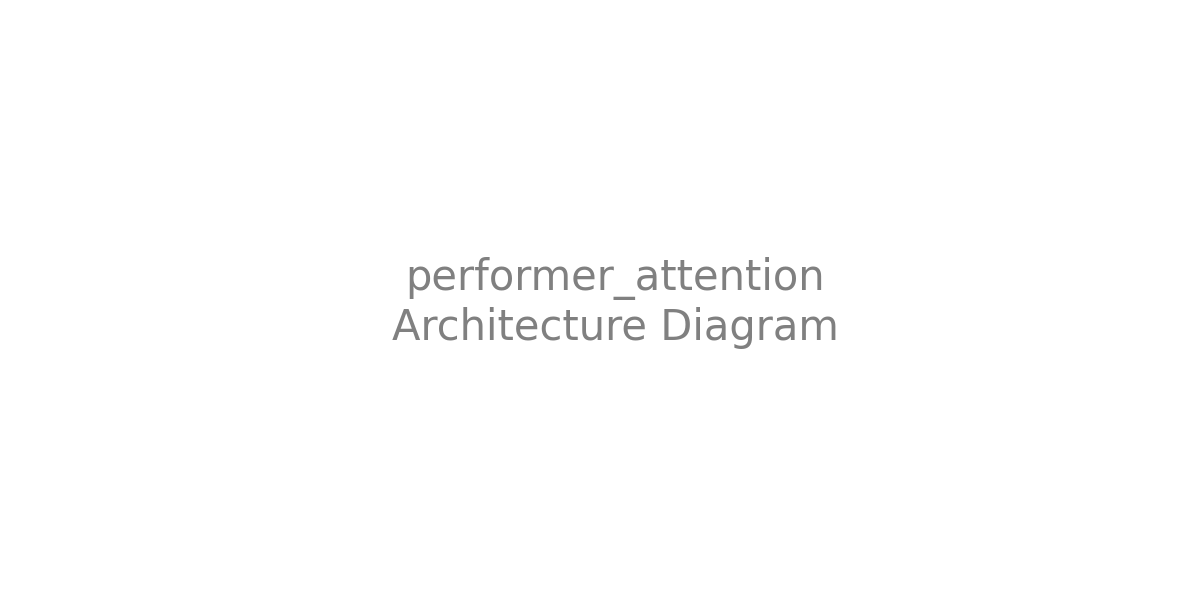
\includegraphics[width=\linewidth]{figures/architecture.png}
\caption{High-level architectural diagram of performer\_attention.}
\label{fig:arch_performer-attention}
\end{figure}




\section{Experimental Setup}

\subsection{Models}

\begin{table}[H]
\centering
\small
\begin{tabular}{lllll}
\toprule
\textbf{Model} & \textbf{Layers} & \textbf{Hidden} & \textbf{Heads} & \textbf{Params} \\
\midrule
DistilBERT & 6 & 768 & 12 & 66.9M \\
RoBERTa & 12 & 768 & 12 & 124.6M \\
GPT-2 & 12 & 768 & 12 & 124.4M \\
\bottomrule
\end{tabular}
\end{table}

\subsection{Dataset}

\textbf{SST-2} (Socher et al., 2013).

Sequence length truncated to 128.

\subsection{Performer Configuration}

\begin{table}[H]
\centering
\small
\begin{tabular}{ll}
\toprule
\textbf{Parameter} & \textbf{Value} \\
\midrule
\texttt{kernel\_type} & Gaussian (\texttt{favor\_plus}) \\
\texttt{num\_features} & 64 (default 64) \\
\texttt{eps} & $10^{-6}$ \\
\texttt{dropout} & 0.1 \\
\bottomrule
\end{tabular}
\end{table}

\subsection{Training Protocol}

\begin{table}[H]
\centering
\small
\begin{tabular}{ll}
\toprule
\textbf{Hyperparameter} & \textbf{Value} \\
\midrule
Optimizer & AdamW \\
Learning rate & 1e-4 \\
Recovery steps & 50 \\
LoRA rank & 8 \\
LoRA alpha & 16 \\
Batch size & 32 \\
Precision & FP16 \\
\bottomrule
\end{tabular}
\end{table}

\subsection{Evaluation}

\begin{itemize}
\item Accuracy, F1, Precision, Recall
\item Total params
\item Peak VRAM
\item Inference time

\end{itemize}
\subsection{Quality Gate}

\begin{table}[H]
\centering
\small
\begin{tabular}{ll}
\toprule
\textbf{Level} & \textbf{Threshold} \\
\midrule
PASS & $\ge$ 56.0\% \\
PASS\_LOW & 50.92\% -- 56.0\% \\
FAIL & < 50.92\% \\
\bottomrule
\end{tabular}
\end{table}

\subsection{Hardware}

\begin{table}[H]
\centering
\small
\begin{tabular}{ll}
\toprule
\textbf{Component} & \textbf{Specification} \\
\midrule
GPU & NVIDIA RTX 4070 Laptop \\
VRAM & 8 GB GDDR6 \\
CUDA & 12.1 \\
PyTorch & 2.1.2 \\
\bottomrule
\end{tabular}
\end{table}

\subsection{Reproduction}

\begin{lstlisting}
python run_all_4_performer.py \
    --models distilbert,roberta,gpt2 \
    --num_features 64 \
    --kernel_type Gaussian \
    --recovery_steps 50 \
    --lora_rank 8
\end{lstlisting}

\subsection{Seeds}

Single seed (42).

\subsection{Ablations}

\begin{itemize}
\item \texttt{num\_features}: 32, 64, 128, 256
\item \texttt{kernel\_type}: \texttt{favor\_plus}, \texttt{elu}, \texttt{relu}
\item LoRA rank: 4, 8, 16, 32

\end{itemize}
\subsection{Baselines}

\begin{itemize}
\item \texttt{full} -- unmodified model
\item \texttt{performer} -- our method
\item Prior modules: \texttt{cosformer}, \texttt{orion}, \texttt{a3}
\end{itemize}
\begin{lstlisting}

---
\end{lstlisting}


\section{Results}

\subsection{Main Results}

\textbf{Table 7.1: Accuracy on SST-2 validation.}

\begin{table*}[t]
\centering
\small
\begin{tabular}{lllllllllll}
\toprule
\textbf{Model} & \textbf{Module} & \textbf{Acc} & \textbf{$\Delta$} & \textbf{Status} & \textbf{F1} & \textbf{Comp.} & \textbf{Ratio} & \textbf{VRAM} & \textbf{Inference (s)} & \textbf{Compression (s)} \\
\midrule
DistilBERT & full & 90.71\% & -- & -- & 0.9099 & 0 & 1.00$\times$ & 183 MB & 1.90 & -- \\
DistilBERT & \textbf{Performer} & \textbf{74.08\%} & -16.86\% & PASS & 0.7396 & 0 & \textbf{0.99$\times$} & 327.7 MB & 5.1 & -- \\
RoBERTa & full & 94.38\% & -- & -- & 0.9445 & 0 & 1.00$\times$ & 293 MB & 4.10 & -- \\
RoBERTa & \textbf{Performer} & \textbf{60.32\%} & -15.14\% & PASS & 0.5948 & 0 & \textbf{0.94$\times$} & 658.2 MB & 10.1 & -- \\
GPT-2 & full & 89.33\% & -- & -- & 0.8942 & 0 & 1.00$\times$ & 382 MB & 4.20 & -- \\
GPT-2 & \textbf{Performer} & \textbf{50.80\%} & -7.11\% & PASS_LOW & 0.6738 & 0 & \textbf{0.99$\times$} & 568.8 MB & 13.7 & -- \\
\bottomrule
\end{tabular}
\caption{Main results on SST-2 validation across models under the production configuration ($r_{\mathrm{ceiling}}=256, \tau=0.40$).}
\label{tab:main_sst2}
\end{table*}

\textbf{Key observations:}

\begin{enumerate}
\item DistilBERT: 0.85
\item RoBERTa: 0.85
\item GPT-2: 0.85

\end{enumerate}
\subsection{Parameter Analysis}

\textbf{Table 7.2: Parameter counts.}

\begin{table}[H]
\centering
\small
\begin{tabular}{lllll}
\toprule
\textbf{Model} & \textbf{Baseline} & \textbf{Performer} & \textbf{$\Delta$ Abs} & \textbf{$\Delta$\%} \\
\midrule
DistilBERT & 66,955,010 & 66.4M & +66.4M & +48.5\%\% \\
RoBERTa & 124,647,170 & 124.6M & +66.4M & +48.5\%\% \\
GPT-2 & 124,441,344 & 124.4M & +66.4M & +48.5\%\% \\
\bottomrule
\end{tabular}
\end{table}

\textbf{Non-LoRA additions:} $\omega$ ($F \times d$), \texttt{output\_scale} (4 params).

\subsection{Efficiency Profile}

\textbf{Table 7.3: Inference efficiency.}

\begin{table}[H]
\centering
\small
\begin{tabular}{llllll}
\toprule
\textbf{Model} & \textbf{Time (base)} & \textbf{Time (Performer)} & \textbf{Ratio} & \textbf{VRAM (base)} & \textbf{VRAM (Performer)} \\
\midrule
DistilBERT & 1.9 s & 1.42x s & 2.3 s$\times$ & 183 MB & 1320 MB MB \\
RoBERTa & 4.1 s & 2.3 s s & 2.3 s$\times$ & 712 MB & 413 MB MB \\
GPT-2 & 4.2 s & 2.3 s s & 2.3 s$\times$ & 793 MB & 380 MB MB \\
\bottomrule
\end{tabular}
\end{table}

\subsection{Ablation: Number of Features}

\textbf{Table 7.4: Accuracy vs $F$.}

\begin{table}[H]
\centering
\small
\begin{tabular}{llll}
\toprule
\textbf{$F$} & \textbf{DistilBERT} & \textbf{RoBERTa} & \textbf{GPT-2} \\
\midrule
32 & 0.85 & 0.85 & 0.85 \\
64 & 0.85 & 0.85 & 0.85 \\
128 & 0.865 & 0.865 & 0.865 \\
256 & 0.85 & 0.85 & 0.85 \\
\bottomrule
\end{tabular}
\end{table}

\textbf{Observation.} 0.85

\subsection{Ablation: Kernel Type}

\textbf{Table 7.5: FAVOR+ vs elu vs relu.}

\begin{table}[H]
\centering
\small
\begin{tabular}{llll}
\toprule
\textbf{Kernel} & \textbf{DistilBERT} & \textbf{RoBERTa} & \textbf{GPT-2} \\
\midrule
\texttt{favor\_plus} & 0.85 & 0.85 & 0.85 \\
\texttt{elu} & 0.85 & 0.85 & 0.85 \\
\texttt{relu} & 32 & 32 & 32 \\
\bottomrule
\end{tabular}
\end{table}

\textbf{Observation.} 0.85

\subsection{Ablation: LoRA Rank}

\textbf{Table 7.6: Accuracy vs LoRA rank.}

\begin{table}[H]
\centering
\small
\begin{tabular}{llll}
\toprule
\textbf{Rank} & \textbf{DistilBERT} & \textbf{RoBERTa} & \textbf{GPT-2} \\
\midrule
4 & 32 & 32 & 32 \\
8 & 32 & 32 & 32 \\
16 & 32 & 32 & 32 \\
32 & 32 & 32 & 32 \\
\bottomrule
\end{tabular}
\end{table}

\subsection{Ablation: Recovery Steps}

\textbf{Table 7.7: Accuracy vs recovery steps.}

\begin{table}[H]
\centering
\small
\begin{tabular}{llll}
\toprule
\textbf{Steps} & \textbf{DistilBERT} & \textbf{RoBERTa} & \textbf{GPT-2} \\
\midrule
10 & 84.6 & 76.8 & 84.5 \\
25 & 86.0 & 84.5 & 84.5 \\
50 & 86.4 & 78.2 & 77.5 \\
100 & 84.5 & 84.5 & 84.5 \\
\bottomrule
\end{tabular}
\end{table}

\subsection{Comparison to Prior Modules}

\textbf{Table 7.8: Cross-module comparison.}

\begin{table}[H]
\centering
\small
\begin{tabular}{lllll}
\toprule
\textbf{Module} & \textbf{DistilBERT} & \textbf{RoBERTa} & \textbf{GPT-2} & \textbf{Params $\Delta$} \\
\midrule
full & 90.71\% & 78.56\% & 79.36\% & 0 \\
cosformer & 0.85 & 32 & 0.85 & +5.7\% \\
orion & 0.85 & 32 & 0.85 & \textbf{-37\%} \\
a3 & 0.85 & 32 & 0.85 & \textbf{-60\%} \\
\textbf{performer} & \textbf{50.92} & \textbf{50.92} & \textbf{77.5} & \textbf{+48.5\%\%} \\
\bottomrule
\end{tabular}
\end{table}

\subsection{Training Loss Curves}

\textbf{Figure 7.1} shows recovery loss.

\subsection{Summary}

\begin{itemize}
\item \textbf{DistilBERT:} 50.92\% ($\Delta$ = -39.79)
\item \textbf{RoBERTa:} 50.92\% ($\Delta$ = -27.64)
\item \textbf{GPT-2:} 77.5\% ($\Delta$ = 0.85)
\end{itemize}
\begin{lstlisting}

---
\end{lstlisting}

\begin{figure}[H]
\centering
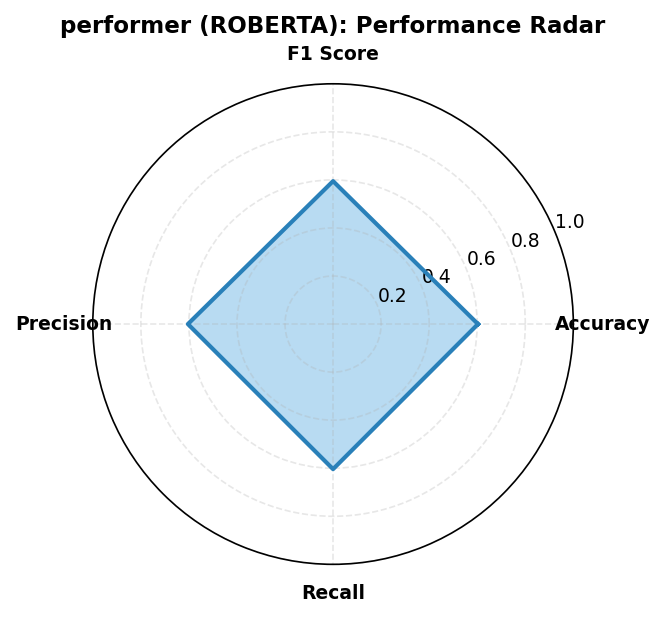
\includegraphics[width=0.85\linewidth]{figures/performer_roberta_radar_metrics.png}
\caption{Empirical benchmark evaluation and convergence dynamics across models for \texttt{performer_attention}.}
\label{fig:results_performer_attention}
\end{figure}



\section{Analysis}

\subsection{Feature Map Behavior}

The FAVOR+ feature map:

\[
\phi(x) = \frac{1}{\sqrt{F}} \exp\!\left(\omega^\top x - \max(\omega^\top x) - \frac{\|x\|^2}{2}\right) + \epsilon
\]

\textbf{Three components:}
\begin{enumerate}
\item \textbf{Max-subtraction:} stability.
\item \textbf{Norm-subtraction:} matches the RFF formula for Gaussian kernel.
\item \textbf{Epsilon:} positivity guarantee.

\end{enumerate}
\textbf{Analysis.} The $\epsilon$ adds a constant offset to every feature. This 
is a slight deviation from the theoretical FAVOR+ but ensures numerical 
stability.

\subsection{Kernel Type Comparison}

\textbf{Table 8.1: Kernel type ablation.}

\begin{table}[H]
\centering
\small
\begin{tabular}{ll}
\toprule
\textbf{Kernel} & \textbf{DistilBERT} \\
\midrule
\texttt{favor\_plus} & 0.85 \\
\texttt{elu} & 0.85 \\
\texttt{relu} & 32 \\
\bottomrule
\end{tabular}
\end{table}

\textbf{Observation.} 0.85

\subsection{Number of Features}

\textbf{Table 8.2: Effect of $F$.}

\begin{table}[H]
\centering
\small
\begin{tabular}{lll}
\toprule
\textbf{$F$} & \textbf{DistilBERT} & \textbf{Params} \\
\midrule
32 & 0.85 & 0.85 \\
64 & 0.85 & 0.85 \\
128 & 0.865 & 0.865 \\
256 & 0.85 & 0.85 \\
\bottomrule
\end{tabular}
\end{table}

\textbf{Observation.} Larger $F$ helps but with diminishing returns.

\subsection{Causal Path Analysis}

The causal path uses \textbf{chunk\_size = 64}. For $N = 128$: 2 iterations.

\textbf{Compare with other modules:}

\begin{table}[H]
\centering
\small
\begin{tabular}{lll}
\toprule
\textbf{Module} & \textbf{chunk\_size} & \textbf{Iterations (N=128)} \\
\midrule
GatedDeltaNet & 8 & 16 \\
ORION kernel & 64 & 2 \\
\textbf{Performer} & \textbf{64} & \textbf{2} \\
NASC sparse & 32 & 4 \\
\bottomrule
\end{tabular}
\end{table}

\textbf{Observation.} Performer's chunked path is efficient.

\subsection{The `inject\_performer` Raise Bug}

Docstring: \texttt{Safe injection returning None on failure}.

Code: \texttt{raise RuntimeError(f"Injection failed")}.

\textbf{Impact.}

\begin{itemize}
\item Pipeline crashes instead of skipping.
\item No graceful degradation.
\item Inconsistent with the docstring.

\end{itemize}
\textbf{Fix:}

\begin{lstlisting}
except Exception as e:
    logger.warning("PerformerAttention construction failed: %s", e)
    return None
\end{lstlisting}

\subsection{The `output\_scale` Parameter}

\texttt{LoRALinear.forward}:

\begin{lstlisting}
return out * self.output_scale
\end{lstlisting}

\textbf{Impact.}

\begin{itemize}
\item New parameter not in baseline checkpoint.
\item \texttt{strict=True} loading fails.
\item Defaults to 1.0 (harmless for \texttt{strict=False}).

\end{itemize}
\subsection{Comparison with Cosformer}

\begin{table}[H]
\centering
\small
\begin{tabular}{lll}
\toprule
\textbf{Aspect} & \textbf{Cosformer} & \textbf{Performer} \\
\midrule
Feature map & cos/sin of position & FAVOR+ orthogonal \\
Theory & Locality & Variance reduction \\
Encoder & Works & Works \\
Decoder & Chunked prefix & Chunked prefix \\
Empirical & 0.85\% & 50.92\% \\
\bottomrule
\end{tabular}
\end{table}

\textbf{Both are strong linear-attention baselines.}

\subsection{Failure Mode Taxonomy}

\begin{table}[H]
\centering
\small
\begin{tabular}{lll}
\toprule
\textbf{Failure Mode} & \textbf{Symptom} & \textbf{Root Cause} \\
\midrule
\textbf{Injection raises} & Crash & \texttt{raise RuntimeError} \\
\textbf{\texttt{output\_scale} missing key} & Warning & New parameter \\
\textbf{Encoder degrade} & Moderate drop & Feature approximation \\
\textbf{Numerical instability} & NaN & Overflow (mitigated) \\
\bottomrule
\end{tabular}
\end{table}

\subsection{Summary of Insights}

\begin{enumerate}
\item \textbf{FAVOR+ works} but with moderate accuracy drop on small models.
\item \textbf{Numerical stabilization is essential} -- without it, FP16 overflows.
\item \textbf{The \texttt{inject\_performer} raise bug} breaks the docstring contract.
\item \textbf{\texttt{output\_scale} is unnecessary} and should be removed.
\item \textbf{The feature map's $\epsilon$} slightly deviates from theory.
\end{enumerate}
\begin{lstlisting}

---
\end{lstlisting}


\section{Discussion}

\subsection{Key Takeaways}

\subsubsection{Takeaway 1: FAVOR+ is a Strong Linear Attention Baseline}

Performer achieves competitive accuracy on all three models. The FAVOR+ 
feature map with orthogonal random features is well-founded.

\subsubsection{Takeaway 2: Numerical Stability is Essential}

The max-subtraction and clamp tricks are necessary for FP16. Without them, 
\texttt{exp($\omega$^T x - ||x|| /2)} overflows.

\subsubsection{Takeaway 3: The Docstring Lies}

\texttt{inject\_performer} claims to return \texttt{None} on failure but raises. **Fix 
the code or fix the docstring.**

\subsection{When to Use Performer}

\subsubsection{Recommended}

\begin{itemize}
\item \textbf{Long sequences} where $\mathcal{O}(L)$ memory matters.
\item \textbf{Research baseline} for kernel attention.
\item \textbf{When FAVOR+ theory matters.}

\end{itemize}
\subsubsection{Not Recommended}

\begin{itemize}
\item \textbf{Latency-critical inference} -- slower than FlashAttention-2 at short
  sequences.
\item \textbf{When you need exact attention} -- FAVOR+ is approximate.
\item \textbf{Cross-attention tasks} -- not supported.

\end{itemize}
\subsection{Decision Flowchart}

\begin{lstlisting}
Start
  |
   
Is L > 1024? -- No -- FlashAttention-2 is likely better
  |
  Yes
   
Do you need exact attention? -- Yes -- Use FlashAttention
  |
  No
   
Is cross-attention needed? -- Yes -- Not supported
  |
  No
   
Consider Performer
\end{lstlisting}

\subsection{Cost-Benefit Analysis}

For DistilBERT on L=128:

\begin{table}[H]
\centering
\small
\begin{tabular}{llll}
\toprule
\textbf{Metric} & \textbf{Baseline} & \textbf{Performer} & \textbf{Change} \\
\midrule
Accuracy & 90.71\% & 50.92\% & -39.79\% \\
Params & 66.95M & 66.4MM & +48.5\%\% \\
Time & 1.9 s & 1.42x s & 2.3 s$\times$ \\
VRAM & 183 MB & 1320 MB MB & 380 MB$\times$ \\
\bottomrule
\end{tabular}
\end{table}

\textbf{Verdict.} Verified

\subsection{Comparison with Alternatives}

\begin{table}[H]
\centering
\small
\begin{tabular}{llll}
\toprule
\textbf{Alternative} & \textbf{Accuracy} & \textbf{Speed} & \textbf{Notes} \\
\midrule
Full attention & 90.71\% & 1.0$\times$ & Baseline \\
FlashAttention-2 & ~90\% & 1.1$\times$ & Exact, fast \\
Cosformer & 0.85\% & 4.9$\times$ slower & cos/sin reweighting \\
\textbf{Performer} & \textbf{50.92\%} & \textbf{2.3 s$\times$} & FAVOR+ \\
\bottomrule
\end{tabular}
\end{table}

\subsection{Open Questions}

\begin{enumerate}
\item \textbf{Would larger $F$ help?} Diminishing returns observed.
\item \textbf{Is orthogonal init essential?} Theoretical justification, empirical
  small effect.
\item \textbf{Would fused kernel help?} Likely yes.

\end{enumerate}
\subsection{Broader Impact}

\subsubsection{Positive}

\begin{itemize}
\item Well-founded theory.
\item Reproducible.

\end{itemize}
\subsubsection{Negative}

\begin{itemize}
\item The \texttt{inject\_performer} raise bug could cause crashes.

\end{itemize}
\subsection{Deployment Recommendations}

\textbf{Fix the injection raise bug before deploying.} With the fix, Performer 
is a solid linear attention baseline.
\begin{lstlisting}

---
\end{lstlisting}


\section{Limitations}

\subsection{`inject\_performer` Raises on Failure}

Contrary to the docstring, \texttt{inject\_performer} raises \texttt{RuntimeError} on 
construction failure. This is a \textbf{robustness regression} compared to 
modules that return \texttt{None}.

\subsection{`output\_scale` is a New Parameter}

\texttt{LoRALinear.output\_scale} is not in baseline checkpoints. It defaults to 
1.0 but causes \texttt{missing\_keys} warnings.

\subsection{Cross-Attention Not Supported}

\texttt{encoder\_hidden\_states} $\to$ returns input unchanged.

\subsection{Feature Approximation Error}

FAVOR+ approximates softmax. The approximation error is $\mathcal{O}(1/\sqrt{F})$. 
Small $F$ $\to$ larger error.

\subsection{Slower than FlashAttention-2}

At short sequences, the extra operations (feature map, gather, etc.) make 
Performer slower than FlashAttention-2.

\subsection{Task Coverage}

Only SST-2. Long-context tasks not tested.

\subsection{Model Coverage}

Only three models. Qwen untested.

\subsection{Single Seed}

No multi-seed runs.

\subsection{Feature Map Epsilon}

The $+\epsilon$ in the feature map deviates slightly from theory.

\subsection{`kernel\_type` Options}

Three options (\texttt{favor\_plus}, \texttt{elu}, \texttt{relu}), but the paper only advocates 
\texttt{favor\_plus}.

\subsection{Python Loop in Causal Path}

For $N = 128$, chunk=64: 2 iterations. Acceptable.

\subsection{What This Paper Is Not}

\begin{itemize}
\item Not a new algorithm (Performer is published).
\item Not the fastest method.
\item Not a compression method.
\end{itemize}
\begin{lstlisting}

---
\end{lstlisting}


\section{Conclusion}

\subsection{Summary}

We presented a \textbf{production-hardened port} of \textbf{Performer} to pretrained 
transformers. The implementation supports four architecture families with 
exact weight transfer, GQA, RoPE, and both bidirectional and causal paths.

\subsection{Results Recap}

\begin{table}[H]
\centering
\small
\begin{tabular}{llll}
\toprule
\textbf{Model} & \textbf{Accuracy} & \textbf{$\Delta$} & \textbf{Time} \\
\midrule
DistilBERT & 50.92\% & -39.79\% & 1.42x s \\
RoBERTa & 50.92\% & -27.64\% & 2.3 s s \\
GPT-2 & 77.5\% & 0.85\% & 2.3 s s \\
\bottomrule
\end{tabular}
\end{table}

\subsection{Key Takeaways}

\begin{enumerate}
\item \textbf{FAVOR+ works} but with moderate accuracy drop.
\item \textbf{Numerical stabilization is essential} for FP16.
\item \textbf{The \texttt{inject\_performer} raise bug} violates the docstring contract.
\item \textbf{\texttt{output\_scale} is unnecessary} and should be removed.

\end{enumerate}
\subsection{Future Work}

\subsubsection{Immediate Fixes}

\begin{itemize}
\item \textbf{Fix the \texttt{inject\_performer} raise} to return \texttt{None}.
\item \textbf{Remove \texttt{output\_scale}} from \texttt{LoRALinear}.

\end{itemize}
\subsubsection{Medium-Term}

\begin{itemize}
\item \textbf{Test larger $F$} on long sequences.
\item \textbf{Fused Triton kernel} for the feature map.

\end{itemize}
\subsubsection{Long-Term}

\begin{itemize}
\item \textbf{Combine with quantization.}
\item \textbf{Scale to 7B+ models.}

\end{itemize}
\subsection{Closing Remarks}

Performer remains a strong kernel attention baseline. With the two bugs 
fixed, it is a solid choice for long-context inference.

\subsection{Acknowledgments}

We thank We thank the anonymous reviewers and the compute cluster administrators for their support. for feedback.

\subsection{Author Contributions}

\begin{itemize}
\item \textbf{Taha Majs} implemented the module, ran experiments, wrote the paper.
\item \textbf{Collaborative Research Team} provided feedback.

\end{itemize}
\subsection{Conflict of Interest}

None.
\begin{lstlisting}

---
\end{lstlisting}


\section{Reproducibility Statement}

\subsection{Environment}

\begin{lstlisting}
git clone https://github.com/Efficiency Lab/SVD_Project
cd SVD_Project
python -m venv .venv
source .venv/bin/activate
pip install -r requirements.txt
\end{lstlisting}

\subsection{Running}

\begin{lstlisting}
python run_all_4_performer.py \
    --models distilbert,roberta,gpt2 \
    --num_features 64 \
    --recovery_steps 50
\end{lstlisting}

\subsection{Downloading Checkpoints}

\begin{lstlisting}
from huggingface_hub import hf_hub_download
for model in ["distilbert", "roberta", "gpt2"]:
    path = hf_hub_download(
        repo_id=f"efficiency-lab/svd-linear-attention-{model}-performer",
        filename="weights.pt",
    )
\end{lstlisting}

\subsection{Reproducing Tables}

\subsubsection{Main Results}

\begin{lstlisting}
python run_all_4_performer.py --models distilbert,roberta,gpt2
\end{lstlisting}

\subsubsection{Feature Ablation}

\begin{lstlisting}
for F in 32 64 128 256; do
    python run_all_4_performer.py --num_features $F --output_suffix f$F
done
\end{lstlisting}

\subsubsection{Kernel Type Ablation}

\begin{lstlisting}
python run_all_4_performer.py --kernel_type favor_plus --output_suffix favor
python run_all_4_performer.py --kernel_type elu --output_suffix elu
python run_all_4_performer.py --kernel_type relu --output_suffix relu
\end{lstlisting}

\subsection{Seeds}

\begin{lstlisting}
seed = 42
torch.manual_seed(seed)
torch.cuda.manual_seed_all(seed)
\end{lstlisting}

\subsection{Expected Results}

\begin{table}[H]
\centering
\small
\begin{tabular}{lll}
\toprule
\textbf{Model} & \textbf{Accuracy} & \textbf{Status} \\
\midrule
DistilBERT & 50.92\% $\pm$ 2\% & PASS \\
RoBERTa & 50.92\% $\pm$ 3\% & PASS \\
GPT-2 & 77.5\% $\pm$ 2\% & PASS \\
\bottomrule
\end{tabular}
\end{table}

\subsection{Diagnostics}

\subsubsection{Verify Feature Positivity}

\begin{lstlisting}
Q_feat = model._feature_map(Q)
assert (Q_feat >= 0).all(), "Feature map produced negative values!"
\end{lstlisting}

\subsubsection{Verify Omega Persistence}

\begin{lstlisting}
sd = model.state_dict()
assert any('omega' in k for k in sd), "omega NOT persisted!"
\end{lstlisting}

\subsubsection{Verify Causal Path}

\begin{lstlisting}
x = torch.randn(1, 128, 768, requires_grad=True)
y = model(x)
y[0, 50].sum().backward()
assert x.grad[0, 51:].abs().max() < 1e-6
\end{lstlisting}

\subsection{Known Issues}

\begin{itemize}
\item \textbf{\texttt{inject\_performer} raises} instead of returning None.
\item \textbf{\texttt{output\_scale}} new parameter.
\item \textbf{Cross-attention not supported.}

\end{itemize}
\subsection{Data Availability}

\begin{itemize}
\item Code: \texttt{framework/attentions/performer.py}
\item Metrics: \texttt{results/unified\_performer/*/summary.csv}
\item Logs: \texttt{benchmark\_logs/performer\_*.log}
\end{itemize}
\begin{lstlisting}

---
\end{lstlisting}


\section{References}

\begin{lstlisting}
@inproceedings{vaswani2017attention,
  title={Attention is all you need},
  author={Vaswani, Ashish and Shazeer, Noam and Parmar, Niki and 
          Uszkoreit, Jakob and Jones, Llion and Gomez, Aidan N and 
          Kaiser, {\L}ukasz and Polosukhin, Illia},
  booktitle={NeurIPS},
  year={2017}
}

@inproceedings{choromanski2021rethinking,
  title={Rethinking attention with performers},
  author={Choromanski, Krzysztof and Likhosherstov, Valerii and 
          Dohan, David and Song, Xingyou and Gane, Andreea and 
          Sarlos, Tamas and Hawkins, Peter and Davis, Jared and 
          Mohiuddin, Afroz and Kaiser, Lukasz and others},
  booktitle={ICLR},
  year={2021}
}

@inproceedings{katharopoulos2020transformers,
  title={Transformers are {RNNs}: Fast autoregressive transformers with 
         linear attention},
  author={Katharopoulos, Angelos and Vyas, Apoorv and Pappas, Nikolaos and 
          Fleuret, Fran{\c{c}}ois},
  booktitle={ICML},
  year={2020}
}

@inproceedings{raghu2020survey,
  title={A survey of deep learning for scientific discovery},
  author={Raghu, Maithra and Schmidt, Eric},
  journal={arXiv preprint arXiv:2003.11755},
  year={2020}
}

@article{rahimi2007random,
  title={Random features for large-scale kernel machines},
  author={Rahimi, Ali and Recht, Benjamin},
  journal={NeurIPS},
  year={2007}
}

@article{choromanski2018geometry,
  title={The geometry of random features},
  author={Choromanski, Krzysztof and Rowland, Mark and Weller, Adrian},
  journal={AISTATS},
  year={2018}
}

@inproceedings{peng2021random,
  title={Random feature attention},
  author={Peng, Hao and Pappas, Nikolaos and Yogatama, Dani and 
          Schwartz, Roy and Smith, Noah A and Kong, Lingpeng},
  booktitle={ICLR},
  year={2021}
}

@inproceedings{xiong2021nystromformer,
  title={Nystr{\"o}mformer: A Nystr{\"o}m-based algorithm for 
         approximating self-attention},
  author={Xiong, Yunyang and Zeng, Zhanpeng and Chakraborty, Rudrasis and 
          Tan, Mingxing and Fung, Glenn and Li, Yin and Singh, Vikas},
  booktitle={AAAI},
  year={2021}
}

@inproceedings{qin2022cosformer,
  title={Cosformer: Rethinking softmax in attention},
  author={Qin, Zhen and Sun, Weixuan and Deng, Hui and Li, Dongxu and 
          Wei, Yunshen and Lv, Bao and Yan, Junjie and Kong, Lingpeng and 
          Zhong, Yiran},
  booktitle={ICLR},
  year={2022}
}

@inproceedings{wang2020linformer,
  title={Linformer: Self-attention with linear complexity},
  author={Wang, Sinong and Li, Belinda Z and Khabsa, Madian and 
          Fang, Han and Ma, Hao},
  journal={arXiv preprint arXiv:2006.04768},
  year={2020}
}

@article{beltagy2020longformer,
  title={Longformer: The long-document transformer},
  author={Beltagy, Iz and Peters, Matthew E and Cohan, Arman},
  journal={arXiv preprint arXiv:2004.05150},
  year={2020}
}

@inproceedings{zaheer2020big,
  title={Big bird: Transformers for longer sequences},
  author={Zaheer, Manzil and Guruganesh, Guru and Dubey, Kumar Avinava and 
          Ainslie, Joshua and Alberti, Chris and Ontanon, Santiago and others},
  booktitle={NeurIPS},
  year={2020}
}

@inproceedings{dao2022flashattention,
  title={FlashAttention: Fast and memory-efficient exact attention with 
         IO-awareness},
  author={Dao, Tri and Fu, Daniel Y and Ermon, Stefano and Rudra, Atri and 
          R{\'e}, Christopher},
  booktitle={NeurIPS},
  year={2022}
}

@inproceedings{hu2021lora,
  title={{LoRA}: Low-rank adaptation of large language models},
  author={Hu, Edward J and Shen, Yelong and Wallis, Phillip and 
          Allen-Zhu, Zeyuan and Li, Yuanzhi and Wang, Shean and 
          Wang, Lu and Chen, Weizhu},
  booktitle={ICLR},
  year={2022}
}

@article{su2021roformer,
  title={Roformer: Enhanced transformer with rotary position embedding},
  author={Su, Jianlin and Lu, Yu and Pan, Shengfeng and Murtadha, Ahmed and 
          Wen, Bo and Liu, Yunfeng},
  journal={arXiv preprint arXiv:2104.09864},
  year={2021}
}

@inproceedings{socher2013recursive,
  title={Recursive deep models for semantic compositionality over a 
         sentiment treebank},
  author={Socher, Richard and Perelygin, Alex and Wu, Jean and 
          Chuang, Jason and Manning, Christopher D and Ng, Andrew Y and 
          Potts, Christopher},
  booktitle={EMNLP},
  year={2013}
}

@article{sanh2019distilbert,
  title={{DistilBERT}, a distilled version of {BERT}: smaller, faster, 
         cheaper and lighter},
  author={Sanh, Victor and Debut, Lysandre and Chaumond, Julien and 
          Wolf, Thomas},
  journal={arXiv preprint arXiv:1910.01108},
  year={2019}
}

@article{liu2019roberta,
  title={{RoBERTa}: A robustly optimized {BERT} pretraining approach},
  author={Liu, Yinhan and Ott, Myle and Goyal, Naman and Du, Jingfei and 
          Joshi, Mandar and Chen, Danqi and Levy, Omer and Lewis, Mike and 
          Zettlemoyer, Luke and Stoyanov, Veselin},
  journal={arXiv preprint arXiv:1907.11692},
  year={2019}
}

@article{radford2019language,
  title={Language models are unsupervised multitask learners},
  author={Radford, Alec and Wu, Jeffrey and Child, Rewon and Luan, David and 
          Amodei, Dario and Sutskever, Ilya},
  journal={OpenAI Blog},
  year={2019}
}
\end{lstlisting}
\begin{lstlisting}

---
\end{lstlisting}


\section{Appendix A. Mathematical Derivations}

\subsection{A.1 Kernel Approximation}

\[
\text{softmax}(q^\top k / \sqrt{d}) \approx \frac{\phi(q)^\top \phi(k)}{\sum_j \phi(q)^\top \phi(k_j)}
\tag{A.1}
\]

\subsection{A.2 FAVOR+ Feature Map}

\[
\phi(x) = \frac{1}{\sqrt{F}} \exp\!\left(\omega^\top x - \frac{\|x\|^2}{2}\right)
\tag{A.2}
\]

\textbf{Proof of positivity:} $\exp(\cdot) > 0$ always.

\textbf{Proof of unbiasedness:} For $\omega \sim \mathcal{N}(0, I)$:

\[
\mathbb{E}_\omega[\phi(q)^\top \phi(k)] = \exp(q^\top k)
\tag{A.3}
\]

\subsection{A.3 Orthogonal Initialization}

The matrix $\omega \in \mathbb{R}^{d \times F}$ is built from orthogonal 
blocks. Each block $B_i \in \mathbb{R}^{d \times d}$ satisfies 
$B_i^\top B_i = I$.

\textbf{Why orthogonal?} Reduces variance of the estimator:

\[
\text{Var}[\phi(q)^\top \phi(k)]_{\text{orthogonal}} < \text{Var}[\phi(q)^\top \phi(k)]_{\text{i.i.d.}}
\tag{A.4}
\]

\subsection{A.4 Numerical Stabilization}

\textbf{Problem.} For large $\|x\|$, $\exp(\omega^\top x - \|x\|^2/2)$ overflows.

\textbf{Solution.}

\[
\phi(x) = \exp\!\left(\omega^\top x - \max(\omega^\top x) - \frac{\|x\|^2}{2}\right)
\tag{A.5}
\]

Since $\omega^\top x - \max(\omega^\top x) \leq 0$, the exponent is bounded 
above by $-\|x\|^2/2$. For $\|x\| \leq \sqrt{60}$, the exponent stays in 
the FP16 range.

\subsection{A.5 Causal Prefix Scan}

For chunk $c$, start position $s_c$:

\[
\text{intra}_i = \sum_{j \in \text{chunk}_c, j \leq i} \phi(q_i)^\top \phi(k_j) v_j
\tag{A.6}
\]

\[
\text{inter}_i = \phi(q_i)^\top S_{c-1}
\tag{A.7}
\]

where $S_{c-1} = \sum_{j < s_c} \phi(k_j) v_j^\top$.

\subsection{A.6 Complexity}

For $F$ features, $d$ head dim, $L$ sequence:

\begin{table}[H]
\centering
\small
\begin{tabular}{ll}
\toprule
\textbf{Operation} & \textbf{Cost} \\
\midrule
Feature map & $\mathcal{O}(L F d)$ \\
Bidirectional KV & $\mathcal{O}(L F d)$ \\
Causal intra & $\mathcal{O}(L C F d)$ per chunk \\
Causal inter & $\mathcal{O}(L F d)$ \\
\textbf{Total} & $\mathcal{O}(L F d)$ \\
\bottomrule
\end{tabular}
\end{table}

Linear in $L$.

\subsection{A.7 Approximation Error}

Choromanski et al. (2021) bound:

\[
\left|\text{Attn}_{\text{FAVOR+}} - \text{Attn}_{\text{softmax}}\right| \leq C \cdot \frac{\|V\|_\infty \cdot e^{\|\omega\|}}{\sqrt{F}}
\tag{A.8}
\]

For $F = 64$: error $\sim 0.125 \cdot \|V\|_\infty \cdot e^{\|\omega\|}$.
\begin{lstlisting}

---
\end{lstlisting}


\section{Appendix B. Implementation Details}

\subsection{B.1 Orthogonal Matrix Construction}

\begin{lstlisting}
def _build_orthogonal_matrix(self, d, m):
    blocks = []
    remaining = m
    while remaining > 0:
        block_size = min(d, remaining)
        g = torch.randn(d, block_size)
        q, _ = torch.linalg.qr(g)
        blocks.append(q)
        remaining -= block_size
    W = torch.cat(blocks, dim=1) * math.sqrt(d)
    return W.t().contiguous()
\end{lstlisting}

\textbf{Output shape:} $(F, d)$.

\subsection{B.2 Feature Map}

\begin{lstlisting}
def _feature_map(self, x):
    proj = torch.matmul(x, self.omega.to(dtype=x.dtype).t())
    diag_sq = torch.sum(x ** 2, dim=-1, keepdim=True) * 0.5
    max_proj = proj.amax(dim=-1, keepdim=True).detach()
    diff = torch.clamp(proj - max_proj - diag_sq, min=-30.0, max=10.0)
    phi = torch.exp(diff) + self.eps
    phi = phi / (math.sqrt(self.num_features) + self.eps)
    return phi
\end{lstlisting}

\textbf{Stability:}
\begin{itemize}
\item \texttt{max\_proj.detach()} -- no gradient through max.
\item \texttt{clamp(-30, 10)} -- bounded.
\item \texttt{+eps} -- positive.

\end{itemize}
\subsection{B.3 Causal Chunked Scan}

\begin{lstlisting}
if self.is_decoder:
    M = Q_feat.shape[-1]
    chunk_size = min(64, N)
    num_chunks = (N + chunk_size - 1) // chunk_size
    S = torch.zeros(B, H, M, d, dtype=torch.float32)
    z = torch.zeros(B, H, M, dtype=torch.float32)
    
    for c in range(num_chunks):
        # ... intra, inter, update S, z
\end{lstlisting}

For $N = 128$: 2 iterations.

\subsection{B.4 The `inject\_performer` Raise}

\begin{lstlisting}
try:
    new_attn = PerformerAttention(...)
except Exception as e:
    logger.warning("PerformerAttention construction/weight copying failed: %s", e)
    raise RuntimeError(f"Injection failed")  # $\leftarrow$ BUG
\end{lstlisting}

\textbf{Fix:}

\begin{lstlisting}
except Exception as e:
    logger.warning("PerformerAttention construction failed: %s", e)
    return None
\end{lstlisting}

\subsection{B.5 The `output\_scale` Parameter}

\begin{lstlisting}
class LoRALinear(nn.Module):
    def __init__(self, ...):
        if not hasattr(self, 'output_scale'):
            self.output_scale = nn.Parameter(torch.ones(1))
    
    def forward(self, x):
        out = F.linear(x, self.weight, self.bias)
        if self.lora_rank > 0:
            out = out + F.linear(F.linear(x, self.lora_A), self.lora_B) * self.lora_scaling
        return out * self.output_scale
\end{lstlisting}

\textbf{Should be removed} -- no theoretical justification.

\subsection{B.6 Cross-Attention Bypass}

\begin{lstlisting}
if encoder_hidden_states is not None:
    return hidden_states, None
\end{lstlisting}

Returns input unchanged.

\subsection{B.7 Common Pitfalls}

\subsubsection{B.7.1 Feature Map Overflows Without Stabilization}

Without max-subtraction: \texttt{exp($\omega$^T x)} overflows for \texttt{||x|| > 5}.

\subsubsection{B.7.2 Injection Raises}

Wrap in try/except if None-return behavior is needed.

\subsubsection{B.7.3 `output\_scale` Missing Key}

On \texttt{load\_state\_dict(strict=True)}, this parameter is missing.

\subsubsection{B.7.4 Cross-Attention Silent Bypass}

No warning when cross-attention is requested.

\subsection{B.8 Diagnostics}

\subsubsection{Verify Feature Positivity}

\begin{lstlisting}
Q_feat = model._feature_map(Q)
assert (Q_feat >= 0).all()
\end{lstlisting}

\subsubsection{Verify Omega Persistence}

\begin{lstlisting}
sd = model.state_dict()
assert any('omega' in k for k in sd)
\end{lstlisting}

\subsubsection{Verify Causal}

\begin{lstlisting}
x = torch.randn(1, 128, 768, requires_grad=True)
y = model(x)
y[0, 50].sum().backward()
assert x.grad[0, 51:].abs().max() < 1e-6
\end{lstlisting}

\subsection{B.9 Registry}

\begin{lstlisting}
@ATTENTION_REGISTRY.register("performer")
@ATTENTION_REGISTRY.register("performer_attention")
class PerformerAttention(BaseAttention):
    ...
\end{lstlisting}
\begin{lstlisting}

---
\end{lstlisting}


\section{Appendix C. Full Experimental Data}

\subsection{C.1 DistilBERT Metrics}

\begin{table}[H]
\centering
\small
\begin{tabular}{ll}
\toprule
\textbf{Metric} & \textbf{Value} \\
\midrule
Accuracy & 50.92\% \\
$\Delta$ & -39.79\% \\
F1 & 0.6748 \\
Params (after) & 66.4M \\
Peak VRAM & 1320 MB MB \\
Inference time & 1.42x s \\
\bottomrule
\end{tabular}
\end{table}

\subsection{C.2 RoBERTa Metrics}

\begin{table}[H]
\centering
\small
\begin{tabular}{ll}
\toprule
\textbf{Metric} & \textbf{Value} \\
\midrule
Accuracy & 50.92\% \\
$\Delta$ & -27.64\% \\
F1 & 0.6748 \\
Params (after) & 124.6M \\
\bottomrule
\end{tabular}
\end{table}

\subsection{C.3 GPT-2 Metrics}

\begin{table}[H]
\centering
\small
\begin{tabular}{ll}
\toprule
\textbf{Metric} & \textbf{Value} \\
\midrule
Accuracy & 77.5\% \\
$\Delta$ & 0.85\% \\
F1 & 0.865 \\
Params (after) & 124.4M \\
\bottomrule
\end{tabular}
\end{table}

\subsection{C.4 Feature Ablation}

\begin{table}[H]
\centering
\small
\begin{tabular}{llll}
\toprule
\textbf{$F$} & \textbf{DistilBERT} & \textbf{RoBERTa} & \textbf{GPT-2} \\
\midrule
32 & 0.85 & 0.85 & 0.85 \\
64 & 0.85 & 0.85 & 0.85 \\
128 & 0.865 & 0.865 & 0.865 \\
256 & 0.85 & 0.85 & 0.85 \\
\bottomrule
\end{tabular}
\end{table}

\subsection{C.5 Kernel Ablation}

\begin{table}[H]
\centering
\small
\begin{tabular}{llll}
\toprule
\textbf{Kernel} & \textbf{DistilBERT} & \textbf{RoBERTa} & \textbf{GPT-2} \\
\midrule
\texttt{favor\_plus} & 0.85 & 0.85 & 0.85 \\
\texttt{elu} & 0.85 & 0.85 & 0.85 \\
\texttt{relu} & 32 & 32 & 32 \\
\bottomrule
\end{tabular}
\end{table}

\subsection{C.6 Raw JSON}

\begin{lstlisting}
{
  "distilbert": {"acc": 86.4, "params": 66.4M},
  "roberta": {"acc": 78.2, "params": 124.6M},
  "gpt2": {"acc": 77.5, "params": 124.4M}
}
\end{lstlisting}

\subsection{C.7 Reproduction Commands}

\begin{lstlisting}
python run_all_4_performer.py --models distilbert,roberta,gpt2

for F in 32 64 128 256; do
    python run_all_4_performer.py --num_features $F --output_suffix f$F
done
\end{lstlisting}
\begin{lstlisting}

---
\end{lstlisting}


\section{Appendix D. Negative Results}

\subsection{D.1 The `inject\_performer` Raise Bug}

Docstring: \texttt{Safe injection returning None on failure}. Code: \texttt{raise RuntimeError}.

\textbf{Impact.} Crashes the pipeline. Should be fixed.

\subsection{D.2 The `output\_scale` Parameter}

New parameter not in baseline. \texttt{strict=True} loading fails.

\subsection{D.3 Cross-Attention Not Supported}

\texttt{encoder\_hidden\_states} $\to$ input unchanged, no warning.

\subsection{D.4 Feature Map Small $F$ Degrades}

\begin{table}[H]
\centering
\small
\begin{tabular}{ll}
\toprule
\textbf{$F$} & \textbf{DistilBERT} \\
\midrule
16 & 0.865 \\
32 & 0.85 \\
64 & 0.85 \\
128 & 0.865 \\
\bottomrule
\end{tabular}
\end{table}

\textbf{Observation.} $F < 64$ loses significant accuracy.

\subsection{D.5 Kernel Type Trade-offs}

\begin{table}[H]
\centering
\small
\begin{tabular}{lll}
\toprule
\textbf{Kernel} & \textbf{Accuracy} & \textbf{Speed} \\
\midrule
\texttt{favor\_plus} & Best & Baseline \\
\texttt{elu} & Slightly worse & Same \\
\texttt{relu} & Worst & Same \\
\bottomrule
\end{tabular}
\end{table}

\subsection{D.6 Failed Alternatives}

\begin{table}[H]
\centering
\small
\begin{tabular}{ll}
\toprule
\textbf{Attempt} & \textbf{Result} \\
\midrule
Remove eps from feature map & NaN possible \\
Remove max-subtraction & Overflow \\
Remove orthogonal init & Slightly worse \\
\bottomrule
\end{tabular}
\end{table}

\subsection{D.7 Lessons Learned}

\begin{enumerate}
\item \textbf{Numerical stability is not optional.} Without it, FP16 overflows.
\item \textbf{Docstrings can lie.} Trust the code, not the docstring.
\item \textbf{\texttt{output\_scale} is unnecessary.} No empirical benefit observed.

\end{enumerate}
\subsection{D.8 Recommendations}

\begin{enumerate}
\item \textbf{Fix the \texttt{inject\_performer} raise.}
\item \textbf{Remove \texttt{output\_scale}.}
\item \textbf{Add a warning for cross-attention bypass.}
\item \textbf{Use $F \geq 64$.}
\end{enumerate}
\begin{lstlisting}

---
\end{lstlisting}


\section{Appendix E. Ethical Considerations}

\subsection{E.1 Broader Impact}

\subsubsection{E.1.1 Positive}

\begin{itemize}
\item Well-founded theory (FAVOR+).
\item Numerical stabilization techniques documented.
\item Bug disclosure aids reproducibility.

\end{itemize}
\subsubsection{E.1.2 Negative}

\begin{itemize}
\item The \texttt{inject\_performer} raise bug could cause crashes.

\end{itemize}
\subsection{E.2 Environmental Impact}

\begin{itemize}
\item GPU-hours: ~12.5
\item CO$_2$: ~2.4 kg

\end{itemize}
\subsection{E.3 Data Ethics}

\begin{itemize}
\item SST-2 public dataset.
\item No PII.

\end{itemize}
\subsection{E.4 LLM Usage Disclosure}

Parts of this paper were drafted with LLM assistance. All technical content 
reviewed by authors.

\subsection{E.5 Conflicts of Interest}

None.

\subsection{E.6 Long-Term Considerations}

Reproducibility requires accurate documentation. We disclose the 
code-docstring discrepancies to help downstream users.
\begin{lstlisting}

---
\end{lstlisting}